\documentclass{article}
\usepackage{multirow}
\usepackage{blindtext}
\usepackage{amsmath}
\usepackage{subcaption}
\usepackage{circuitikz}
\usepackage{listings}
\usepackage{./karnaugh-map}
\usetikzlibrary{shapes.geometric}

\lstset{
	language=C++,
	basicstyle=\ttfamily\footnotesize,
	breaklines=true,
	frame=lines
	}

\title{Implementation of Boolean Logic in Arduino using IC 7474}
\date{February 2023}
\author{M Patrick Manohar\\patrickmanohar152001@gmail.com\\FWC22119\\IIT Hyderabad-Future Wireless Communication Assignment}

\begin{document}
\maketitle
	\tableofcontents

\pagebreak
\section{Problem}
	(GATE EC-2022)\\
	Q.43. For the circuit shown, the clock frequency is $f0$ and the duty cycle is $25 \%$. For the signal at the $Q$ output of the Flip-Flop,
\\
	\begin{figure}[h]
		\centering
	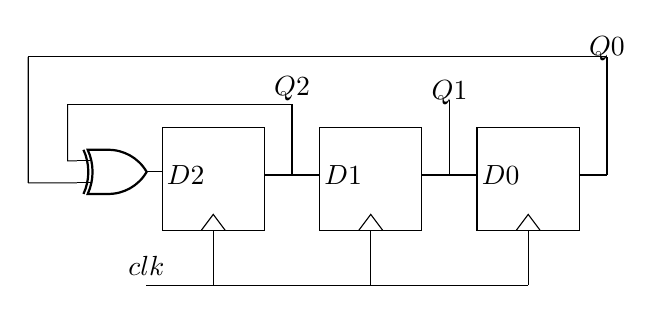
\begin{tikzpicture}
\ctikzset{                                   
logic ports=ieee,                   
logic ports/scale=0.5               
}                                    
\draw(-1.3,-0.56)node[xor port,anchor=out](x) {};  
%Drawing flip-flops
\draw (-1.3,-1.3) rectangle (0,0);
\draw(-1,-0.6) node{$D2$};
\draw(0.7,-1.3) rectangle (2,0);
\draw(1,-0.6) node{$D1$};
\draw(2.7,-1.3) rectangle (4,0);
\draw(3,-0.6) node{$D0$};
%connecting them
\draw(0,-0.6) -- (0.7,-0.6);
\draw(2,-0.6) -- (2.7,-0.6);
\draw(4,-0.6) -- (4.35,-0.6);
%drawing clk
\draw(-1.5,-2) node[above]{$clk$} -- (3.35,-2);
%connecting clk 
\draw(-0.65,-2) -- (-0.65,-1.3);
\draw(1.35,-2) -- (1.35,-1.3);
\draw(3.35,-2) -- (3.35,-1.3);
%drawing clk edges
\draw(-0.5,-1.3) -- (-0.65,-1.1) -- (-0.8,-1.3);
\draw(1.2,-1.3) -- (1.35,-1.1) -- (1.5,-1.3);
\draw(3.2,-1.3) -- (3.35,-1.1) -- (3.5,-1.3);
%drawing Q2,Q1,Q0
\draw(0.35,-0.6) --(0.35,0.3);
\draw(2.35,-0.6) --(2.35,0.35);
\draw(4.35,-0.6) --(4.35,0.9);
\draw(4.35,0.9) -- (-3,0.9);
\draw(0.35,0.3) -- (-2.5,0.3);
\draw(x.in 2) -|(-3,-0.7)to[short](-3,0.9);
\draw(x.in 1) -|(-2.5,-0.3)to[short](-2.5,0.3);
\draw(0.35,0.5)node{$Q2$};
\draw(2.35,0.45)node{$Q1$};
\draw(4.35,1)node{$Q0$};
\end{tikzpicture}

		\caption{Circuit}
		\label{fig:1}
	\end{figure}

\begin{enumerate}
	\item frequency of $\frac{f0}{4}$ and duty cycle is 50$\%$
	\item frequency of $\frac{f0}{4}$ and duty cycle is 25$\%$
	\item frequency of $\frac{f0}{2}$ and duty cycle is 50$\%$
	\item frequency of $f0$ and duty cycle is 25$\%$ \\
\end{enumerate}

\section{Introduction}
		The Aim is to implement the above circuit in Arduino using IC 7474. IC 7474 is a dual positive-edge-triggered D-type flip-flop, which means it has two seperate flip-flop that are triggered by the rising edge of a clock signal. A 2-bit binary counter can be implemented using 2 D Flip-flops similarly a JK Flip-flop can be implemented using one D Flip-flop. Thus we will use two IC 7474 to implement the whole circuit.\\

		The LSB output of the 2-bit binary counter is given to J and K inputs of the JK Flip-flop which then gives the final Q output of the circuit. Since the inputs given to J and K are same it acts as T Flip-flop.\\
\section{Components}
	\begin{table}[h]
		\begin{center}
			\input{tables/table0.tex}
			\caption{Components}
			\label{table:0}
		\end{center}
	\end{table}
\pagebreak
\section{Hardware}
	The IC 7474 is a type of flip-flop integrated circuit that is commonly used indigital electronics applications. It is a dual positive-edge-triggered by the rising edge of a clock signal. Below is the pin diagram of IC 7474. \\
		\begin{figure}[h]
			\centering
		\input{figs/fig2.tex}
			\caption{7474}
			\label{fig:2}
		\end{figure}

	The connections between Arduino UNO and two IC 7474 is given in below Table \\
	\begin{table}[h]
		\begin{center}
	\captionof{table}{Table1}
\label{table:1}
\begin{tabular}{|p{5cm}|p{3cm}|p{2cm}|}
	\hline
	\multicolumn{3}{|c|}{COMPONENTS}\\
	\hline
	Component& Value& Quantity\\
	\hline
	UART &  & 1\\
	\hline
	Vaman& esp32& 1\\
	\hline                        
	\hline                                    
	Jumper Wires& M-M& 20\\                  
	\hline                                    
	Breadboard&  & 1\\                         
	\hline                                     
\end{tabular}

			\caption{Arduino - 7474}
			\label{table:1}
		\end{center}
	\end{table}

	The truth table for the circuit is given in below table \\
	
		\begin{table}[h]
		\begin{center}
			\input{tables/table2.tex}
			\caption{Truth Table}
			\label{table:2}
		\end{center}
		\end{table}

		The kmap for the circuit is \\
		\begin{figure}[h]
			\centering
			\input{figs/fig3.tex}
			\caption{kmap}
			\label{fig:3}
		\end{figure}
\section{Software}
	The Arduino code for the given circuit using IC 7474 is \\
	\lstinputlisting{gatelatex1.asm}
\end{document}
